\documentclass[PhD-Yoann-Dupont.tex]{subfiles}
\begin{document}

Morfessor \citep{creutz2005unsupervised,virpioja2013morfessor} est une famille d'algorithmes créés pour répondre à la tâche de la segmentation morphologique, où les tokens sont découpés en tokens, utilisés à l'origine pour analyser des langues agglutinantes comme le Finnois. La première version de Morfessor, appelée Morfessor Baseline, a été développée par \citet{creutz2002unsupervised}. Diverses variantes en furent créées, notamment Morfessor Categories-MAP \citep{creutz2005inducing} et Allomorfessor \citep{virpioja2009unsupervised}. Les algorithmes Morfessor sont des modèles génératifs probabilistes dont la probabilité marginale est inspirée de la \emph{longueur de description minimale}, \emph{Minimum Description Length} (MDL) en Anglais. La MDL a été décrite par \citet{rissanen1978modeling}, l'idée est de fournir une représentation des données la plus compressée possible. Le principe étant que plus une représentation des données est compressée, mieux elle modélise les régularités présentes dans celles-ci.

Morfessor distingue trois types d'unités. Premièrement, les \emph{atomes} sont les éléments minimaux, ils ne peuvent pas être segmentés, dans notre cas, il s'agit des caractères. Ensuite viennent les \emph{constructions} qui sont des séquences contigües d'atomes qu'il est possible d'accumuler, il s'agit pour nous de \emph{sous-chaînes}. Finalement, les \emph{composants} sont les exemples observés à segmenter, pour une analyse morphologique il s'agit donc des tokens. La segmentation d'un composant en constructions est appelée son \emph{analyse}.

Comme dit au-dessus, Morfessor est une famille de modèles génératifs probabilistes. Il modélise la probabilité de prédire un ensemble de composants W et leurs analyses A selon des paramètres $\theta$ : $p(A, W | \theta)$. Les paramètres $\theta$ du modèle représentent deux éléments : le lexique $\mathcal{L}$ et la grammaire $\mathcal{G}$. Le lexique comprend l'ensemble des constructions, tandis que la grammaire indique comment les constructions peuvent être combinées pour former des composants. L'analyse $a$ d'un composant $w$ est définie par la fonction de segmentation $a = \phi(w;\theta)$.

Selon un ensemble d'apprentissage $D_{w}$ et des paramètres $\theta$, Morfessor optimise une estimation du \emph{maximum a posteriori} (MAP) de la probabilité $p(A, W | \theta)$. Le but est donc de trouver l'ensemble de paramètres $\theta$ le plus probable selon un ensemble d'apprentissage $D_{W}$ :

\begin{equation}
\theta_{MAP} = \argmax{\theta}\ p(\theta | D_{W}) = \argmax{\theta}\ p(\theta)p(D_{W} | \theta)
\end{equation}

La fonction de coût à minimiser étant :

\begin{equation}\label{eq:L-theta}
L(\theta, D_{W}) = -\log p(\theta) - \log p(D_{W} | \theta)
\end{equation}

Il est possible de faire ici l'analogie avec MDL : idéalement, $\theta$ est une représentation condenscée des données dont nous cherchons à minimiser le coût.

\begin{figure}[ht!]
\centering
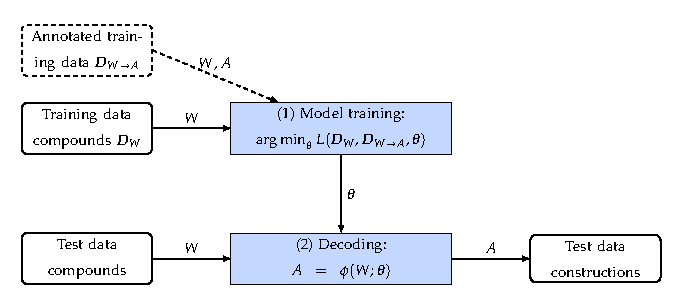
\includegraphics[scale=1.0]{images/morfessor/morfessor-workflow}
\caption{Illustration du workflow global de Morfessor, reprise de \citet{virpioja2013morfessor}. Le modèle est entraîné en optimisant les paramètres $\theta$ minimisant la fonction de coût $L(D_{W}, D_{W \rightarrow A}, \theta)$ selon des composants W dans un ensemble d'entrainement non-annoté $D_{W}$, et optionnellement des composants W et leur construction A dans un ensemble d'entrainement annoté $D_{W \rightarrow A}$. Les paramètres du modèle entraîné servent alors à segmenter les nouvelles données dans la phase de décodage à l'aide de la fonction $\phi$.}
\label{fig:morfessor-workflow}
\end{figure}

L'illustration du workflow de Morfessor est donné dans la figure \ref{fig:morfessor-workflow}. Morfessor utilise un algorithme d'optimisation local ne regardant qu'un seul composant $w_{j}$ à la fois. Il sélectionne d'abord l'analyse minimisant la fonction de coût :

\begin{equation}
y^{(t)}_{j} = \argmin{y_{j} \in Y_{j}} \left \{ min\ L(\theta, Y^{(t-1)}, D_{W}) \right \}
\end{equation}

Où $Y^{t-1}$ est l'ensemble des analyses à un instant t-1. Les paramètres sont alors ajustés selon la formule suivante :

\begin{equation}
\theta(t) = \argmin{\theta} \left \{ L(\theta, Y^{(t)}, D_{W}) \right \}
\end{equation}

La convergence vers un minimum local est garantie du fait qu'aucune des deux fonctions précédentes ne peut augmenter le coût du modèle. En effet, au pire cas, le modèle ne sera tout simplement pas modifié. Un exemple de corpus avec ses composants et les différents segments générés est disponible dans la figure \ref{fig:morfessor-tree}.

\begin{figure}[ht!]
\begin{minipage}{0.33\linewidth}
    \centering
    \begin{tabular}{|l|l|}
    \hline
    compte & token \\
    \hline
    1      & unmatched \\
    1      & matchbox \\
    1      & matched \\
    2      & boxes \\
    5      & match \\
    7      & box \\
    \hline
    \end{tabular}
\end{minipage}
\begin{minipage}{0.66\linewidth}
    \centering
    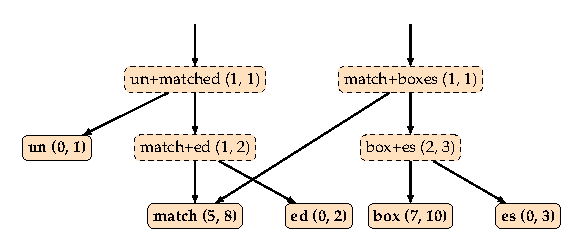
\includegraphics[scale=1.0]{images/morfessor/morfessor-tree}
\end{minipage}
\caption{À gauche, un corpus d'entrée pour Morfessor. À droite, l'arbre d'analyse correspondant au corpus. Les éléments ayant un contour en pointillet sont des éléments pouvant être segmentés, tandis que les éléments avec un contour plein ne le peuvent pas. À chaque élément est associé un couple de nombres (X,Y) : X correspond au nombre d'occurrences d'un élément en tant que composants dans le corpus, Y correspond au nombre d'occurrences accumulées en additionant à X l'ensemble des nombres d'occurrences de l'ensemble des ancêtres de l'élément. Image tirée de \citet{virpioja2013morfessor}.}
\label{fig:morfessor-tree}
\end{figure}

Afin de donner une idée de la compression des données, nous utiliserons la définiton "brute" du principe de MDL de \citet{grunwald2005tutorial} (page 11). Bien que cette mesure ne soit pas exactement celle utilisée par Morfessor, elle s'en inspire et est moins fastidieuse à calculer :

\begin{equation}
L(D,H) = L(H) + L(D|H)
\end{equation}

Où $L(H)$ représente la taille en nombre de bits de H et $L(D|H)$ représente la taille en nombre de bits du corpus encodé selon H (ici, la taille de l'ensemble des analyses). Nous voyons que cette formule est similaire à l'équation \ref{eq:L-theta}. Si nous reprenons la figure \ref{fig:morfessor-tree}, nous avons $D$ défini selon le tableau de gauche. Nous pouvons comparer l'analyse fournie dans la figure \ref{fig:morfessor-tree}, que nous appellerons $H_{1}$ à deux analyses caricaturales des données :

\begin{itemize}
    \item $H_{1}$ : l'analyse fournie dans la figure \ref{fig:morfessor-tree}. $H_{1}$ = \{un, match, ed, box, es\}
    \item $H_{2}$ : l'ensemble des hypothèses est l'ensemble des caractères observés. $H_{2}$ = \{a, b, c, d, e, h, m, n, o, s, t, u, x\}
    \item $H_{3}$ : l'ensemble des hypothèses est l'ensemble des tokens observés. $H_{2}$ = \{unmatched,matchbox,matched,boxes,match,box\}
\end{itemize}

$L(H)$ est la taille en nombre de bits de $H$ :

\begin{equation}
L(H) = \sum_{h \in H} L(h)
\end{equation}

Pour $H_{1}$, nous avons donc $L(H_{1}) = L(un) + L(match) + L(ed) + L(box) + L(es) = 2 + 5 + 2 + 3 + 2 = 14$. De la même manière, nous avons $L(H_{2})=13$ et $L(H_{3})=37$.

$L(D|H)$ est la taille en nombre de bits des analyses :

\begin{equation}
L(D|H) = taille(\phi(d;H))
\end{equation}

Pour $H_{1}$, nous avons donc $L(D|H_{1})$ = $taille(\phi(unmatched;H_{1}))$ +\\$taille(\phi(matchbox;H_{1}))$ + ... + 7 $\times$ $taille(\phi(box;H_{1}))$ = 3 + 2 + ... + 7 $\times$ 1 = 23. De manière équivalente, nous avons $L(D|H_{2}) = 80$ et $L(D|H_{3}) = 17$.

Au final, nous avons donc :

\begin{itemize}
    \item $L(D,H_{1}) = L(H) + L(D|H) = 14 + 23 = 37$
    \item $L(D,H_{2}) = 13 + 80 = 93$
    \item $L(D,H_{3}) = 37 + 17 = 57$
\end{itemize}

L'hypothèse $H_{1}$ permet donc de beaucoup mieux compresser les données que les autres hypothèses. L'hypothèse faite par Morfessor est que cette compression est une meilleure représentation des données d'un point de vue de leur segmentation.

Dans les sections suivantes, nous comparerons Morfessor à nos algorithmes de recherche de sous-chaînes fréquentes dans le cadre de la REN chimique à base de CRF.

\end{document}